% doc_map.tex: Generate map of how Lumiera developer documentation is organised
%  glossary.sh - Lumiera RfC:
%
%  Copyright (C)         Lumiera.org
%    2023,               Benny Lyons <benny.lyons@gmx.net>
%
%  This program is free software; you can redistribute it and/or
%  modify it under the terms of the GNU General Public License as
%  published by the Free Software Foundation; either version 2 of
%  the License, or (at your option) any later version.
%
%  This program is distributed in the hope that it will be useful,
%  but WITHOUT ANY WARRANTY; without even the implied warranty of
%  MERCHANTABILITY or FITNESS FOR A PARTICULAR PURPOSE.  See the
%  GNU General Public License for more details.
%
%  You should have received a copy of the GNU General Public License
%  along with this program; if not, write to the Free Software
%  Foundation, Inc., 675 Mass Ave, Cambridge, MA 02139, USA.

%
% To compile the graphics, you will require TikZ.
% On Debian, this is to be found in the texlive-pictures package.
%
\documentclass[dvisgvm]{article}
\usepackage{tikz}


\begin{document}

\pagestyle{empty}

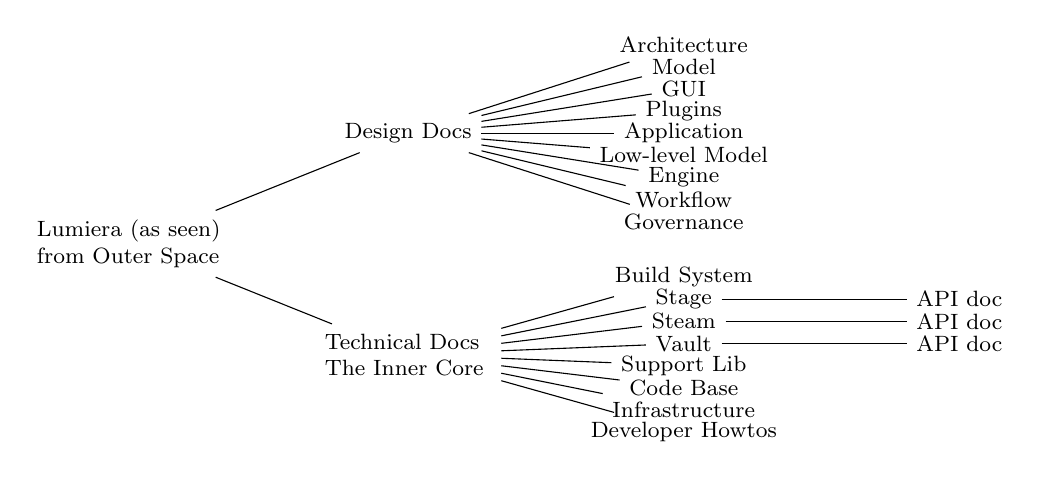
\begin{tikzpicture}
  [font=\footnotesize,
    grow=right,
    level 1/.style={sibling distance=8em},
    level 2/.style={sibling distance=0.8em},level distance=3.5cm]

  \node{\hbox{\vbox{
                \hbox{Lumiera (as seen)}
                \hbox{from Outer Space}
              }
        }
  } % root
  child {node {\hbox{\vbox{
                       \hbox{Technical Docs}
                       \hbox{The Inner Core}
                     }
               }
    }
    child {node {Developer Howtos} }
    child {node {Infrastructure} }
    child {node {Code Base} }
    child {node {Support Lib} }
    child {node {Vault} child { node {API doc}}}
    child {node {Steam} child { node {API doc}}}
    child {node {Stage} child { node {API doc}}}
    child {node {Build System} }
  }
  child {node {Design Docs}
    child {node {Governance} }
    child {node {Workflow} }
    child {node {Engine} }
    child {node {Low-level Model} }
    child {node {Application} }
    child {node {Plugins} }
    child {node {GUI} }
    child {node {Model} }
    child {node {Architecture} }
  };

\end{tikzpicture}



\end{document}
